Chapter \ref{ch:approach} has formalized the problem and put forward out an approach for evaluating how efficiently a vocabulary list may help a human language learner acquire competency, by using the performance of AI models in an NLP task on a corpus as a proxy metric for language ability.
An general approach has also been proposed in chapter \ref{sec:utility-extraction-with-xai} for actually compiling vocabulary lists that approach maximal efficiency.

In this chapter, we will describe possible implementations of this approach, first setting criteria for the selection of its components and then suggestion concrete options.


\section{Data Pipeline}


\section{NLP Tasks}
The choice of NLP tasks employed to test a XAI-based approach for word utility estimation is a crucial step:
Since we are trying to estimate the utility a word a word has to language understanding, the NLP tasks should reflect language understanding as much as possible.
A good place to start looking for such tasks are those which are typically employed for pre-training NLP models:
Pre-training tasks are used to first endow the AI model with a general understanding of the language, before using transfer learning to specialize it for a more specific downstream task.
Such tasks must necessarily be general and require general language understanding, since training the model with them is supposed to provide a solid basis for a wide variety of NLP tasks.
Another benefit of using pre-training tasks is that their training is unsupervised, meaning there is no need to manually label data.
\todo{Look at various pre-training tasks, preferably those used by state-of-the-art AI models}
\todo{include free availability for AI models in their justification}

\subsection{NLP Pre-Training Tasks Used by State-of-the-Art AI Models}
This section takes a look at the pretraining process of recent state-of-the-art LLM models which have made public their training process.
Both the NLP tasks and the kind of data is considered.


\begin{description}
	\item[GPT-4] \cite{openaiGPT4TechnicalReport2024}

	      Task: Language modeling (see next section).

	      Data: Not disclosed in detail, according to the original paper, the model was trained "using both publicly available data (such as internet data) and data licensed from third-party providers".
	\item[GPT-3] \cite{brownLanguageModelsAre2020}
	      GPT-3 is a model that does not rely on transfer learning to apply its linguistic understanding to new tasks; instead, it uses zero-shot and few-shot learning to perform tasks it was not specifically trained for.

	      Task: Language modeling (same as GPT-2 \cite{radfordLanguageModelsAre2019})

	      Data: Common Crawl, WebText2, Books1, Books2, Wikipedia \todo{link sources?}
	\item[LLama 3.3] \cite{LlamamodelsModelsLlama3_3}


	      Task: Meta did not make public the training process for Llama 3.3.

	      Data: "data from publicly available sources"
\end{description}

\subsection{Tasks Considered}
\begin{description}
	\item[Next Sentence Prediction]
	      In this task, the AI model takes as input two sentences and predicts a probability for the second sentence being the successor of the first sentence in their source text.
	      Advantages for this task for our purposes is that such a dataset is easy to generate, as it merely requires a corpus of sentences that follow from each other, which is easily obtained from Wikipedia articles, film subtitles, or any other continuous text.

	\item[Text summarization]
	      This task involves summarizing a given text, in other words, writing a shorter version of the input text while still conveying as much of the information from the original text as possible.
	      Summarizing texts seems to require a high level of "understanding" of the text and would thus seem to be good choice for testing whether ablating certain words from the text would have detrimental effect on the model performance.
	      Unfortunately, this task requires hand-labeled datasets and is thus not a good candidate if we aim to find approaches which can be implemented in many different languages, as there is a dearth in data in many of the less-studied languages of the world.

	\item[Masked language modeling (aka. "cloze task")]
	\item[Causal language modeling (aka. Next token prediction)]
	\item[Sentence order prediction]
	\item[Sentence embeddings]
	      Sentence embeddings take the approach of transforming words into meaningful vectors and extend it to whole sentences.
	      This "task" differs from the others in that we do not measure differences in performance when the input is perturbed; but rather a distance between the embedding vectors themselves.
	      This justification for such an approach is that sentences whose meaning is very different should end up further apart from each other in the vector space once embedded.
	      This brings several advantages:
	      This approach can be performed on any corpus containing distinct sentences.
	      These corpus does not have to be document-level, and sentences need not be consecutive.
	      To make this a task on which XAI methods can be applied, we can define a distance from the original token
\end{description}

\subsection{Sentence Embedding Methods}

\begin{description}
	\item[LASER] \cite{artetxeMassivelyMultilingualSentence2019}
	\item[BERT] \cite{reimersMakingMonolingualSentence2020}
\end{description}

\subsection{Data Required for Each NLP Task}
The various NLP tasks employed require certain types of corpora to be employed properly:

\begin{itemize}
	\item[Next sentence prediction]
	      Requires a corpus that contains consecutive sentences.
	      Furthermore, NSP typically predicts whether two sentences follow each other in a document, not a dialogue (see the data on BERT training \cite{kentonBertPretrainingDeep2019}).
	      This excludes movie subtitles from the possible corpora for this task.

\end{itemize}

\section{XAI Methods}

The XAI methods used in this work are the following:
\begin{itemize}
	\item Attention as Explanation
	      Advantages:
	      Model only needs to be run once per sentence.
	      Longer sentences do not lead to a much longer calculations
	      Disadvantages: Justification as explanation controversial.
	\item Single Token Ablation
\end{itemize}

The following lays out how each of these methods works to achieve the goal of word utility estimation.

\begin{description}
	\item [Performance difference of AI for NLP tasks]
	      Here, a Large Language Model (LLM) or a more specific language processing model is made to run NLP tasks such as text summarization, sentiment detection or question-answering.
	      To find out which words help the AI model the most in performing its tasks, words are methodically omitted from texts and the AI’s performance is recorded.
	      This metric attempts to approximate utility by finding words which, when missing, cause the greatest performance loss in the NLP tasks.
	      Evaluation metrics like Shapley values \cite{wangShapleyExplanationNetworks2021} may be used to measure the impact of missing words
	\item [Transformer attention]
	      The transformer architecture is based on a mechanism called \textit{self-attention}.
	      It allocates the neural network's processing to important parts of the input and thus provides some degree of explainability "out of the box".

	\item [Difference in internal vector representation for AI reading text]
	      This approach words similarly to the above involving an AI model, but instead of measuring the changes in the quality of its output, it measures how much changing the input to the model changes its the internal vector state: AI stores data in vector format, and when performing NLP tasks on texts, there is an internal vector representation.
	      By using various distance metrics, it may be possible to find out which words have the greatest impact on the model’s understanding of a text.
	      Most of these approaches can be done both for individual words and word sequences (n-grams).
	      While individual words are the easiest to examine, sometimes n-grams are insightful for finding sequences of words whose meaning is more than the sum of their parts (idioms and collocations) and which therefore must be learned in separately from their constituents (meaningful English n-grams include e.g. “kick the bucket”, “such that”, “such as”).

	      This also raises the question of what is considered a “word”.
	      A phrase like “such as” can be considered two words if the definition of a word is simply “something separated by a space” or one word if the definition is “a phrase whose meaning cannot be arrived at trivially from knowing the definition of its parts”.
	      In Natural Language Processing, tokenizers break down texts into words, but they typically use the first definition for a word in the case of English.
	      Many non-European language do not use spaces in their spelling (e.g. Japanese, Mandarin Chinese) or use spaces to separate a different unit of text (syllables in Vietnamese, sentences in Thai), making this definition of a word unpractical.
	      In most languages, words can appear in various different forms: Verbs in Spanish are conjugated according to the time and originator of an action, Nouns in German are declined depending on their number and grammatical case.
	      This adds another variable for compiling word lists: Whether the list should consider any different combination of letters as a different word, or whether different forms of the same headword should be viewed as only one word.
\end{description}


\section{Interdependencies Between Components Used}

While the components described above can mostly be used in any combination, there are some important restrictions to keep in mind:

\begin{description}
	\item[Attention as XAI can only be used on transformers]
	\item[Tokenization (and thus selection of word candidates) is only independent on model used in input perturbation approaches]
	      As a direct consequence of this, other XAI mechanisms like attention as explanation are only useful for our purposes if the AI model uses a tokenization approach that somewhat corresponds to human notions of words.
	      If a model uses tokenization approaches where a token is a combination of any three letters, any list obtained that tries to order the tokens by utility, while meaningful, will not be useful for human vocabulary learning.
	      Note that in such cases, we can postprocess the data obtained, by merging the tokens to human-readable words and taking the average or maximum attention score of the AI model's tokens.
	\item[]
\end{description}



\section{AI Models}
\begin{itemize}
	\item NSP-model ABC
	\item LLAMA?
\end{itemize}

\todo{tests of performance tests of models used with corpora used (e.g., if NSP prediction model is reliable)}

\section{Tokenizers}
[explanation of why tokenizers are important, explain various possible definitions of "word"]
[explain why morphosyntactically rich languages necessitate word splitting to some extend]

In some XAI models, we are free to choose any tokenizer we like.
We can choose, for instance, to only use full words, or word parts in English.
In input perturbation XAI approaches, we can choose to mask any part of the input with the help of tokenizers.
For decomposition approaches, the model is not looked at as a black box but instead examined using model-specific methods such as attention or Layer-based Relevance Propagation.
In such approaches, only the calculations made by the model itself are available for analysis, which means we are not free to choose our own word-splitting approach independent from the model.
This is because these models are trained using a specific tokenizer in the preprocessing, and changing the preprocessing makes the model function incorrectly.



\section{Input Data}
\subsection{Selection Criteria}

For the purposes of this paper, it was desirable that the corpora used be:
\begin{itemize}
    \item representative of what language learners strive for
    \item available in many languages
    \item for background corpora: Document-level
    \item freely accessible
\end{itemize}

\subsection{Corpora Used}
\begin{description}
	\item[OpenSubtitles Parallel Corpus]
	      This set of corpora contains parallel corpora:
	      Corpora which has text segments in one language aligned with the presumed translation of the segment in a second language.
	      Its sentences are generated from subtitles from the popular subtitle sharing platform \textit{OpenSubtitles} (https://www.opensubtitles.org/) and undergo various preprocessing and filtering steps as described in \cite{lisonOpensubtitles2016ExtractingLarge2016}.
	      These include:
	      \begin{enumerate}
		      \item Enforcing universal UTF-8 character encoding.
		      \item
		            Splitting and joining of sentences from their original subtitles blocks (the segments which appear on screen when watching the movie with its subtitle).
		            One such block may contain multiple sentences, or only a partial one.
		            There is thus a n-to-m-relationship between the blocks and sentences.
		      \item Checking and correcting possible spelling issues, especially ones arising from OCR (Optical character recognition) errors.
		      \item From available subtitles, identifying the subtitle pair which is most likely to be accurate in its alignments and free from errors such spelling, taking into account metadata such as user ratings of subtitles.

	      \end{enumerate}
		  One advantageous aspect of this corpus is that is contains many sentences that are sequential, which means we can generate a Next Sentence Prediction dataset from it (add hedging here since not all lines in corpus are sequential and even within the same movies there may will be pauses in the subs).
		  This corpus has been used to train machine translation models such as OPUS-MT \cite{tiedemannOPUSMTbuildingOpenTranslation2020}, a freely available set of transformer models for translation, including between low-resource languages. \todo{Not completely correct, the pipeline uses data from OPUS, not necessarily or specifically from OpenSubs}
		  While it is possible to reconstruct which movies the subtitle lines came from from information contained in the corpus, it is unfortunately not clear how these movies were selected in the first place.

	\item[Leipzig Wortschatz Corpora]
		Available in x languages

		But: data quality issues, methodology might be outdated

		\cite{goldhahnBuildingLargeMonolingual2012}
	\item[CCMatrix / NLLB]

\end{description}

The full process, as illustrated by the authors, can be seen in figure \ref{fig:opensubs pipeline}
As of 2025, the latest version of the corpus (v2018) contains aligned subtitles of 62 languages between each other.

\begin{figure}[H]
	\centering
    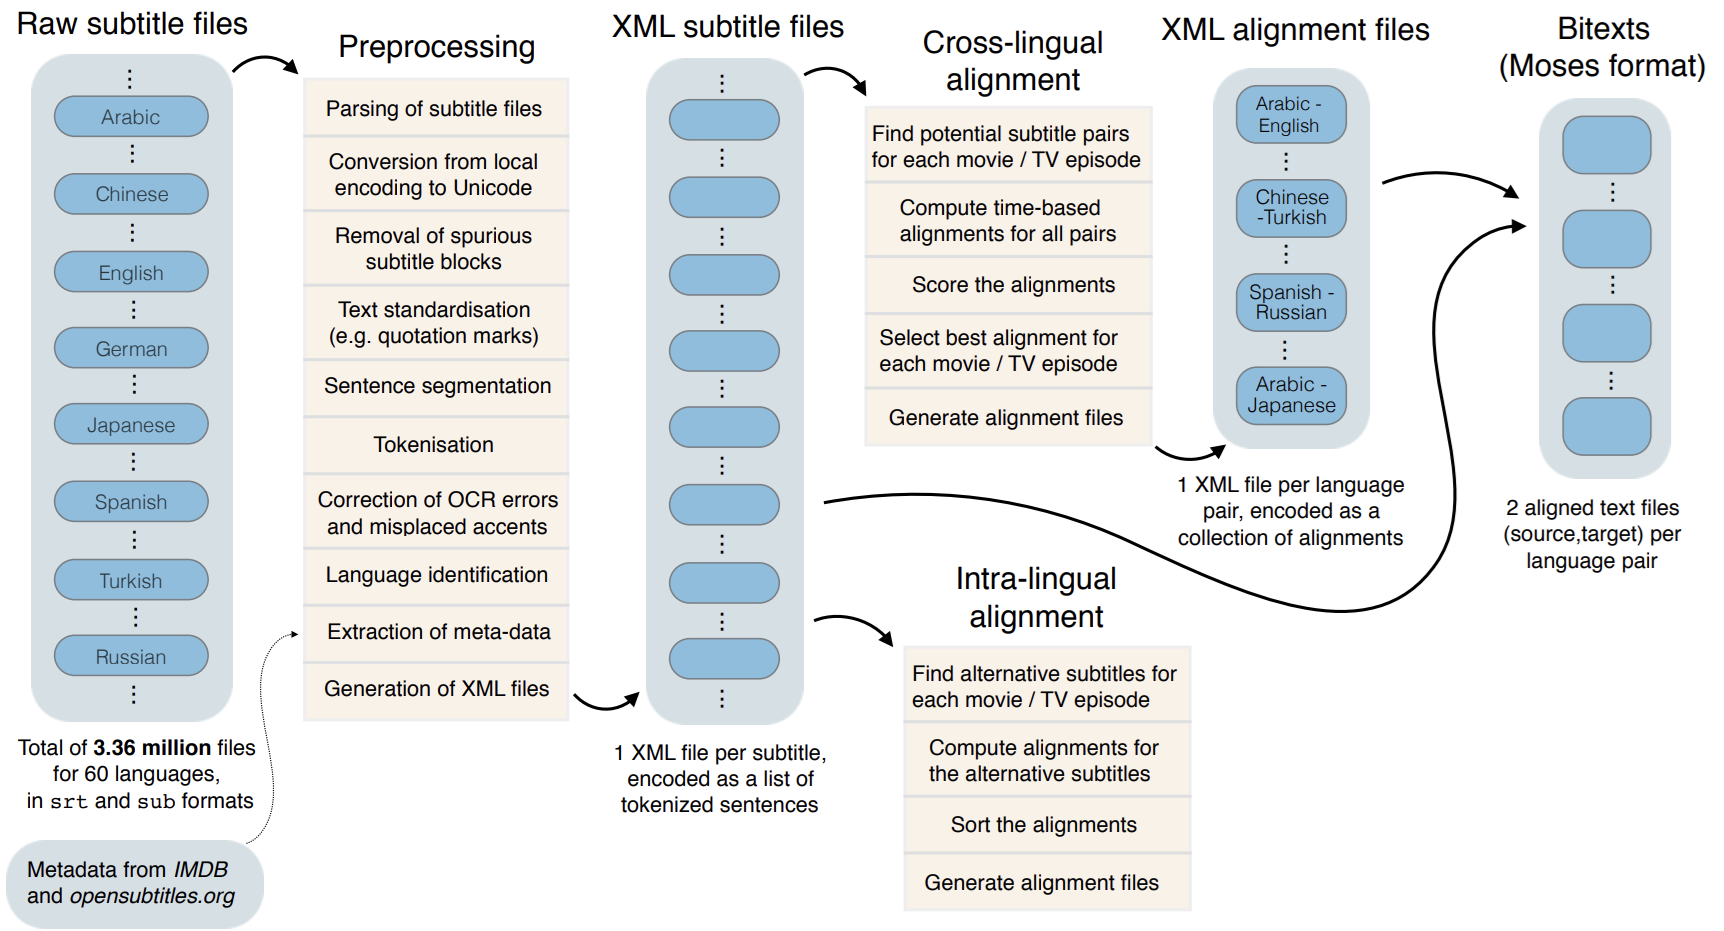
\includegraphics[width=\textwidth]{opensubs_corpus_processing.png}
	\caption{The pipeline producing the OpenSubtitles parallel corpus}
    \label{fig:opensubs pipeline}
\end{figure}


\subsection{Data Augmentation}
Data Augmentation was not used to gain additional data.
While in recent years data augmentation methods have become popular for training AI models in NLP, most of these would have either no or a detrimental effect on the methods employed in this paper:
Some of these methods include \cite{pellicerDataAugmentationTechniques2023}:
\begin{description}
	\item[Character level]
	      Introducing character swaps to data is a method used to train the model to noise in the data, but in our case, would only add noise to the results.
	\item[Word level]
	      There exist techniques to switch words for synonyms or swap words in the sentences to create noise.
	      As with noise on the word level, adding words in inappropriate places is undesired for our use case.
	      Swapping words for synonyms would also prove detrimental, as this would skew the statistics away from the natural word distribution found in the human-generated source texts.
\end{description}
Higher level techniques suffer from the same issues.
For this reason, the data is left in its "natural state" for our purposes.


